% Source: graduate-coursework/Research/Intro_to_Agents/handouts/Part4_Planning_Workflow.tex

\documentclass[border=4pt]{standalone}
\usepackage{graphicx}
\usepackage{tikz}
\usepackage{xcolor}
\usetikzlibrary{shapes.geometric, arrows.meta, positioning, calc, fit, backgrounds}

\definecolor{UofSCGarnet}{HTML}{73000A}
\definecolor{UofSCBlack}{HTML}{000000}
\definecolor{UofSCWhite}{HTML}{FFFFFF}
\definecolor{UofSCAtlantic}{HTML}{466A9F}
\definecolor{UofSCCongaree}{HTML}{1F414D}
\definecolor{UofSCHorseshoe}{HTML}{65780B}
\definecolor{UofSCRose}{HTML}{CC2E40}
\definecolor{UofSCDarkGarnet}{HTML}{570008}
\definecolor{UofSC90Black}{HTML}{363636}
\definecolor{UofSC70Black}{HTML}{5C5C5C}
\definecolor{UofSC50Black}{HTML}{A2A2A2}

\tikzset{
    box/.style={
        draw=UofSCBlack,
        fill=#1,
        minimum width=2.5cm,
        minimum height=0.8cm,
        text=UofSCWhite,
        font=\small\bfseries,
        align=center,
        inner sep=4pt
    },
    box/.default=UofSCGarnet,
    lightbox/.style={
        draw=UofSCBlack,
        fill=UofSCWhite,
        minimum width=2.5cm,
        minimum height=0.8cm,
        text=UofSCBlack,
        font=\small,
        align=center,
        inner sep=4pt
    },
    arrow/.style={
        ->,
        >=Stealth,
        thick,
        UofSCBlack
    },
    bigarrow/.style={
        ->,
        >=Stealth,
        line width=1.5pt,
        UofSCGarnet
    },
    phase/.style={
        draw=UofSCBlack,
        fill=#1,
        minimum width=3cm,
        minimum height=1cm,
        text=UofSCWhite,
        font=\bfseries,
        align=center
    },
    phase/.default=UofSCGarnet,
    subphase/.style={
        draw=UofSC70Black,
        fill=UofSCWhite,
        minimum width=2.8cm,
        minimum height=0.6cm,
        text=UofSCBlack,
        font=\scriptsize,
        align=center
    },
    cyclebox/.style={
        draw=UofSCBlack,
        line width=1.5pt,
        fill=#1,
        minimum width=2cm,
        minimum height=1.2cm,
        text=UofSCWhite,
        font=\bfseries,
        align=center
    },
    cyclebox/.default=UofSCGarnet
}

\begin{document}
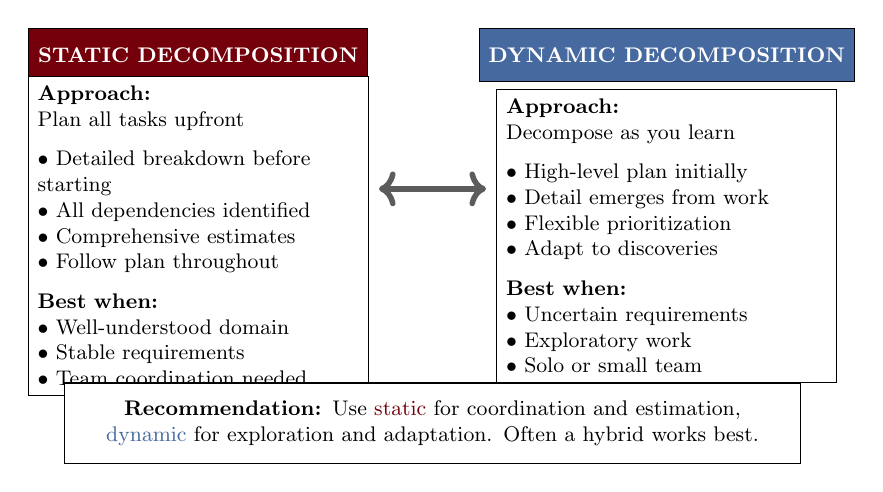
\begin{tikzpicture}[scale=0.85, transform shape]
        % Static side
        \node[box=UofSCGarnet, minimum width=5cm] at (-3.5,3) {STATIC DECOMPOSITION};
        \node[lightbox, minimum width=5cm, minimum height=4cm, text width=4.8cm, align=left] at (-3.5,0.3) {
            \textbf{Approach:}\\
            Plan all tasks upfront\\[0.2cm]
            $\bullet$ Detailed breakdown before starting\\
            $\bullet$ All dependencies identified\\
            $\bullet$ Comprehensive estimates\\
            $\bullet$ Follow plan throughout\\[0.2cm]
            \textbf{Best when:}\\
            $\bullet$ Well-understood domain\\
            $\bullet$ Stable requirements\\
            $\bullet$ Team coordination needed
        };

        % Dynamic side
        \node[box=UofSCAtlantic, minimum width=5cm] at (3.5,3) {DYNAMIC DECOMPOSITION};
        \node[lightbox, minimum width=5cm, minimum height=4cm, text width=4.8cm, align=left] at (3.5,0.3) {
            \textbf{Approach:}\\
            Decompose as you learn\\[0.2cm]
            $\bullet$ High-level plan initially\\
            $\bullet$ Detail emerges from work\\
            $\bullet$ Flexible prioritization\\
            $\bullet$ Adapt to discoveries\\[0.2cm]
            \textbf{Best when:}\\
            $\bullet$ Uncertain requirements\\
            $\bullet$ Exploratory work\\
            $\bullet$ Solo or small team
        };

        % Comparison arrow
        \draw[<->, line width=2pt, UofSC70Black] (-0.8,1) -- (0.8,1);

        % Bottom recommendation
        \node[lightbox, minimum width=11cm, minimum height=1.2cm, text width=10.5cm] at (0,-2.5) {
            \textbf{Recommendation:} Use \textcolor{UofSCGarnet}{static} for coordination and estimation, \textcolor{UofSCAtlantic}{dynamic} for exploration and adaptation. Often a hybrid works best.
        };
    \end{tikzpicture}
\end{document}
